%%%%%%%%%%%%%%%%%%%%%%%%%%%%%%%%%%%%%%%%%
% Jacobs Landscape Poster
% LaTeX Template
% Version 1.1 (14/06/14)
%
% Created by:
% Computational Physics and Biophysics Group, Jacobs University
% https://teamwork.jacobs-university.de:8443/confluence/display/CoPandBiG/LaTeX+Poster
% 
% Further modified by:
% Nathaniel Johnston (nathaniel@njohnston.ca)
%
% This template has been downloaded from:
% http://www.LaTeXTemplates.com
%
% License:
% CC BY-NC-SA 3.0 (http://creativecommons.org/licenses/by-nc-sa/3.0/)
%
%%%%%%%%%%%%%%%%%%%%%%%%%%%%%%%%%%%%%%%%%

%----------------------------------------------------------------------------------------
%	PACKAGES AND OTHER DOCUMENT CONFIGURATIONS
%----------------------------------------------------------------------------------------

\documentclass[final]{beamer}

\usepackage[orientation=landscape,size=a2,scale=1.4]{beamerposter}
%\usepackage[scale=1.24]{beamerposter} % Use the beamerposter package for laying out the poster

\usetheme{confposter} % Use the confposter theme supplied with this template

\setbeamercolor{block title}{fg=ngreen,bg=white} % Colors of the block titles
\setbeamercolor{block body}{fg=black,bg=white} % Colors of the body of blocks
\setbeamercolor{block alerted title}{fg=white,bg=dblue!70} % Colors of the highlighted block titles
\setbeamercolor{block alerted body}{fg=black,bg=dblue!10} % Colors of the body of highlighted blocks
% Many more colors are available for use in beamerthemeconfposter.sty

%-----------------------------------------------------------
% Define the column widths and overall poster size
% To set effective sepwid, onecolwid and twocolwid values, first choose how many columns you want and how much separation you want between columns
% In this template, the separation width chosen is 0.024 of the paper width and a 4-column layout
% onecolwid should therefore be (1-(# of columns+1)*sepwid)/# of columns e.g. (1-(4+1)*0.024)/4 = 0.22
% Set twocolwid to be (2*onecolwid)+sepwid = 0.464
% Set threecolwid to be (3*onecolwid)+2*sepwid = 0.708

\newlength{\sepwid}
\newlength{\onecolwid}
\newlength{\twocolwid}
\newlength{\threecolwid}
\setlength{\sepwid}{0.024\paperwidth} % Separation width (white space) between columns
\setlength{\onecolwid}{0.22\paperwidth} % Width of one column
\setlength{\twocolwid}{0.464\paperwidth} % Width of two columns
\setlength{\threecolwid}{0.708\paperwidth} % Width of three columns
%-----------------------------------------------------------

\usepackage[brazil]{babel}
\usepackage[utf8]{inputenc}
\usepackage{graphicx}  % Required for including images
\graphicspath{{images/}}

\usepackage{booktabs} % Top and bottom rules for tables

%----------------------------------------------------------------------------------------
%	TITLE SECTION 
%----------------------------------------------------------------------------------------

\title{Classificação não-supervisionada hierárquica de artigos jornalísticos} % Poster title

\author{Cirillo Ribeiro Ferreira (cirillo.ferreira@usp.br) Orientador: Prof. Dr. Alair Pereira do Lago} % Author(s)

\institute{Instituto de Matemática e Estatística, Universidade de São Paulo - Trabalho de Formatura Supervisionado} % Institution(s)

%----------------------------------------------------------------------------------------

\begin{document}

\addtobeamertemplate{block end}{}{\vspace*{1ex}} % White space under blocks
\addtobeamertemplate{block alerted end}{}{\vspace*{1ex}} % White space under highlighted (alert) blocks

\setlength{\belowcaptionskip}{1ex} % White space under figures
\setlength\belowdisplayshortskip{1ex} % White space under equations

\begin{frame}[t] % The whole poster is enclosed in one beamer frame

\begin{columns}[t] % The whole poster consists of three major columns, the second of which is split into two columns twice - the [t] option aligns each column's content to the top

\begin{column}{\sepwid}\end{column} % Empty spacer column

\begin{column}{\onecolwid} % The first column

%----------------------------------------------------------------------------------------
%	OBJECTIVES
%----------------------------------------------------------------------------------------

\begin{alertblock}{Objetivos}

Este trabalho tem como objetivos:
\begin{itemize}
\item Estudos das principais classes de algoritmos para agrupamento de documentos textuais.
\item Criação de uma biblioteca para agrupamento de artigos jornalísticos disponíveis nos meios digitais.
\item Proposta e implementação do sistema hVINA (\textit{Hierarchical Viewer of News Articles}) para simplificar a interação entre o usuário e a biblioteca.
\end{itemize}

\end{alertblock}

%----------------------------------------------------------------------------------------
%	INTRODUCTION
%----------------------------------------------------------------------------------------

\begin{block}{Introdução}

Com a criação da internet e a popularização de seu uso como ferramenta de comunicação, houve uma explosão de informação que tornou muito difícil a classificação dos documentos produzidos e publicados nela de maneira manual. A área de classificação de documentos é bem interessante e possui diversas aplicações práticas como classificação de spam, identificação de idioma e análise de sentimento, porém, em especial, artigos jornalísticos têm um enorme desafio devido à grande quantidade de novos documentos criados diariamente e a diversidade de temas abordados. %, especialmente em blogs, mas que carecem de melhor organização.

Para tal propósito serão utilizados algoritmos de aprendizagem não-supervisionadas, pois não necessitam de um conjunto de treinamento como entrada, permitindo o seu uso em conjuntos de dados bem variados, algo que é bem comum em artigos jornalísticos.

\end{block}

%------------------------------------------------

\begin{figure}
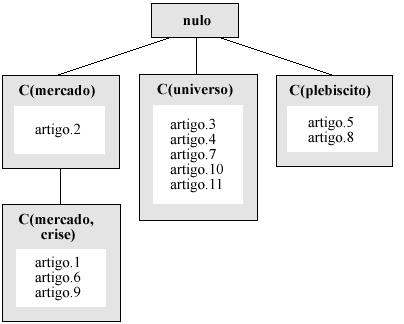
\includegraphics[width=0.5\linewidth]{fihc.png}
\caption{Exemplo de agrupamento feito pelo FIHC}
\end{figure}

%----------------------------------------------------------------------------------------

\end{column} % End of the first column

\begin{column}{\sepwid}\end{column} % Empty spacer column

\begin{column}{\twocolwid} % Begin a column which is two columns wide (column 2)

\begin{columns}[t,totalwidth=\twocolwid] % Split up the two columns wide column

\begin{column}{\onecolwid}\vspace{-.6in} % The first column within column 2 (column 2.1)

%----------------------------------------------------------------------------------------
%	MATERIALS
%----------------------------------------------------------------------------------------

\begin{block}{Análise de agrupamento}

Análise de agrupamento é uma classificação de padrão que emprega o processo de aprendizagem não-supervisionada e tem como objetivo o particionamento de objetos em grupos cujo membros sejam similares entre si e diferentes dos membros de outros grupos \cite{Jain:1999}.

%\begin{enumerate}
%\item Curabitur pellentesque dignissim
%\item Eu facilisis est tempus quis
%\end{enumerate}

\end{block}

\begin{block}{Algoritmos hierárquicos}

Os algoritmos da área de agrupamento são divididos geralmente em duas classes: Algoritmos planos e hierárquicos.
Os algoritmos hierárquicos são aqueles que geram uma árvore de grupos,  uma estrutura que fornece mais informação, uma vez que as relações implícitas entre os grupos ficam mais evidentes.
Há duas abordagens na criação da árvore, a primeira chamada de divisiva ou \textit{top-down} inicia a construção da raiz até as folhas, a segunda chamada de aglomerativa ou \textit{bottom-up} inicia a construção das folhas à raiz.

\end{block}

%----------------------------------------------------------------------------------------
%	MATHEMATICAL SECTION
%----------------------------------------------------------------------------------------

\begin{block}{FIHC}

Foi implementado inicialmente na biblioteca o \textit{Frequent Itemset-based Hierarchical Clustering} (FIHC), que é um algoritmo para agrupamento hierárquico de documentos textuais \cite{Martin:2004} que utiliza o conceito de conjuntos de itens frequentes (\textit{frequent itemset}).

O FIHC está na classe dos algoritmos hierárquicos aglomerativos e baseia-se no seguinte critério de similaridade para a construção da árvore de grupos:

\begin{equation}
Sim(Ci \gets Cj) = \frac{Score(Ci \gets doc(Cj))}{N} + 1
\label{eqn:Sim}
\end{equation}

Onde \textit{Ci} e \textit{Cj} são os grupos usados na comparação de similaridade, \textit{Score} é uma medida de relevância de um documento em um grupo;

\begin{equation}
N = \sum_{x}tfidf(x, doc(Cj)) + \sum_{x'}tfidf(x', doc(Cj))
\label{eqn:Sim_N}
\end{equation}

e \textit{tfidf} é uma medida para avaliação da relevância de uma palavra em um documento.

\end{block}

%----------------------------------------------------------------------------------------

\end{column} % End of column 2.1

\begin{column}{\onecolwid}\vspace{-.6in} % The second column within column 2 (column 2.2)

%----------------------------------------------------------------------------------------
%	METHODS
%----------------------------------------------------------------------------------------

\begin{block}{Conjunto de itens frequentes}
Um conceito importante para o entendimento do FIHC é a noção de conjunto de itens frequentes de uma coleção, cuja definição é: um conjunto de palavras que ocorrem numa quantidade de documentos da coleção acima de um limiar de apoio definido pelo usuário.
\end{block}

\begin{block}{Arquitetura da biblioteca}

A biblioteca abrange todos os passos de uma solução para agrupamento, desde o pré-processamento dos documentos até os algoritmos de agrupamento propriamente ditos. Além disso, foi arquitetada para trabalhar com diversos idiomas. A sua arquitetura é mostrada na figura 2.

\begin{figure}
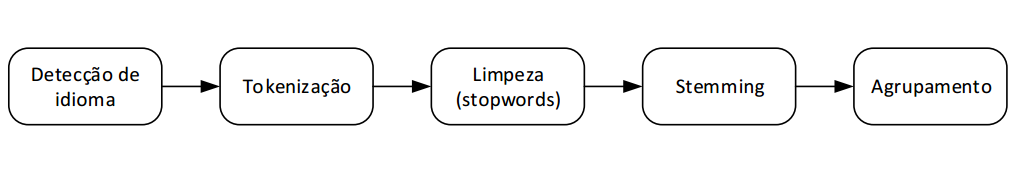
\includegraphics[width=0.95\linewidth]{arquitetura.png}
\caption{Arquitetura proposta para a biblioteca}
\end{figure}

O pré-processamento consiste nos seguintes passos:

\begin{itemize}
\item Detecção de idioma: O primeiro passo para realizar o agrupamento é identificar o idioma utilizado nos documentos, pois os algoritmos dos passos seguintes necessitam desse conhecimento. %Detecta o idioma mais provável da coleção de documentos atráves de método n-grama.
\item Tokenização: Segmenta os textos em palavras.
\item Limpeza: Remove as palavras que possuem pouca relevância no texto, como as preposições, os artigos e marcações gráficas.
\item \textit{Stemming}: Unifica formas variantes de palavras que possuem o mesmo significado, como as palavras ``economia'' e ``econômico''.
\end{itemize}

% Exemplo de negrito \textbf{Donec}

%\end{block}

%----------------------------------------------------------------------------------------
%	RESULTS
%----------------------------------------------------------------------------------------

%\begin{block}{O sistema hVINA}

Já o sistema \textit{hVINA} tem como objetivo criar uma interface amigável para que qualquer usuário possa utilizar a biblioteca, permitindo ao usuário informar uma coleção de artigos de seu interesse ou utilizar coleções pré-selecionadas pelo sistema.


\end{block}

%----------------------------------------------------------------------------------------

\end{column} % End of column 2.2

\end{columns} % End of the split of column 2 - any content after this will now take up 2 columns width

\end{column} % End of the second column

\begin{column}{\sepwid}\end{column} % Empty spacer column

\begin{column}{\onecolwid} % The third column

%----------------------------------------------------------------------------------------
%	CONCLUSION
%----------------------------------------------------------------------------------------

\begin{block}{Conclusão}

A biblioteca desenvolvida é modular, permitindo acrescentar o tratamento de outros idiomas ou implementar novos algoritmos de forma não intrusiva. Ademais, outros projetos além do \textit{hVINA} podem utilizá-la facilmente, visto que ela segue as especificações do distribuidor de pacotes do Ruby (RubyGems).

\begin{figure}
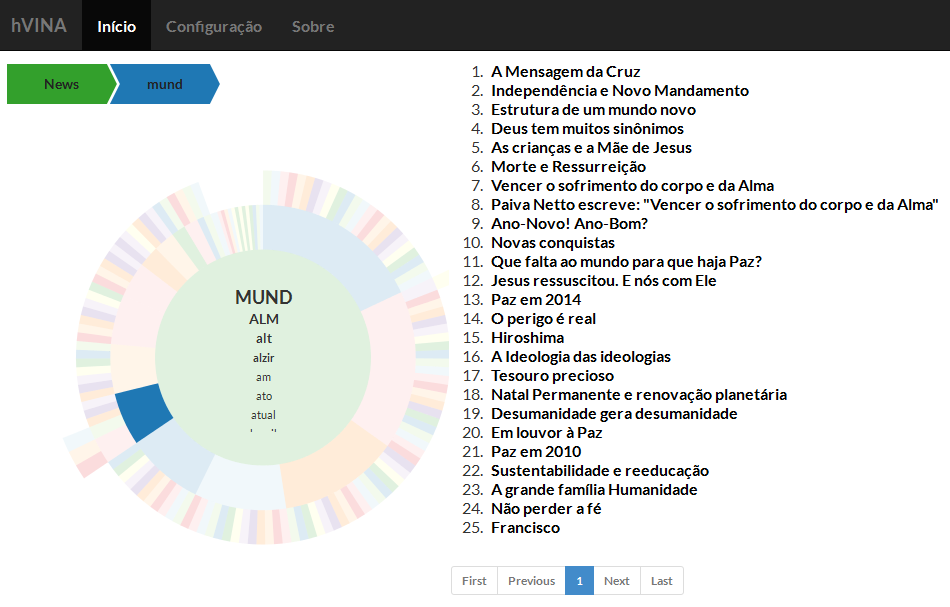
\includegraphics[width=1\linewidth]{hvina.png}
\caption{Tela principal do hVINA}
\end{figure}

O resultado obtido pela biblioteca em conjunto com o sistema \textit{hVINA} demostra a viabilidade de uma solução que tenha boa usabilidade e seja amigável a qualquer usuário, onde não haja a necessidade de treinamento do algoritmo e a configuração seja quase zero.

Porém, melhorias na escalabilidade da biblioteca devem ser feitas nos trabalhos futuros.


%\begin{table}
%\vspace{2ex}
%\begin{tabular}{l l l}
%\toprule
%\textbf{Treatments} & \textbf{Response 1} & \textbf{Response 2}\\
%\midrule
%Treatment 1 & 0.0003262 & 0.562 \\
%Treatment 2 & 0.0015681 & 0.910 \\
%Treatment 3 & 0.0009271 & 0.296 \\
%\bottomrule
%\end{tabular}
%\caption{Table caption}
%\end{table}

\end{block}

%----------------------------------------------------------------------------------------
%	REFERENCES
%----------------------------------------------------------------------------------------

\begin{block}{Referências}

\nocite{*} % Insert publications even if they are not cited in the poster
\small{\bibliographystyle{unsrt}
\bibliography{sample}}

\end{block}

%----------------------------------------------------------------------------------------
%	ACKNOWLEDGEMENTS
%----------------------------------------------------------------------------------------

\begin{center}
\begin{tabular}{ccc}

\includegraphics[width=0.2\linewidth]{IME.png} & \hfill & 
\includegraphics[width=0.4\linewidth]{USP.jpg}
\end{tabular}
\end{center}

%----------------------------------------------------------------------------------------

\end{column} % End of the third column

\begin{column}{\sepwid}\end{column} % Empty spacer column

\end{columns} % End of all the columns in the poster

\end{frame} % End of the enclosing frame

\end{document}